After three months time, the app developed has been successful in addressing YoungDrive's goals with the app, with very high precision to the needs and context of the end users. In figure~\ref{fig:iteration-map} the app development from iteration 1-4 are shown. The final app works on web or as an app, online or offline, on all of YoungDrive's Android and iOS devices. The app is fast to use, the back button on the phone can be used to go to the previous view, and the font size and images are consistent for each screen (which was not the case iteration 1-3, see figure \ref{fig:iteration-map} E-3. The goal was to provide a great learning experience, with a strong YoungDrive feel (embracing the values of fun, plus using the YoungDrive logo and colors).

  \todo{Flytta bild till helsida!}
  \begin{figure}[h]
    \centering
    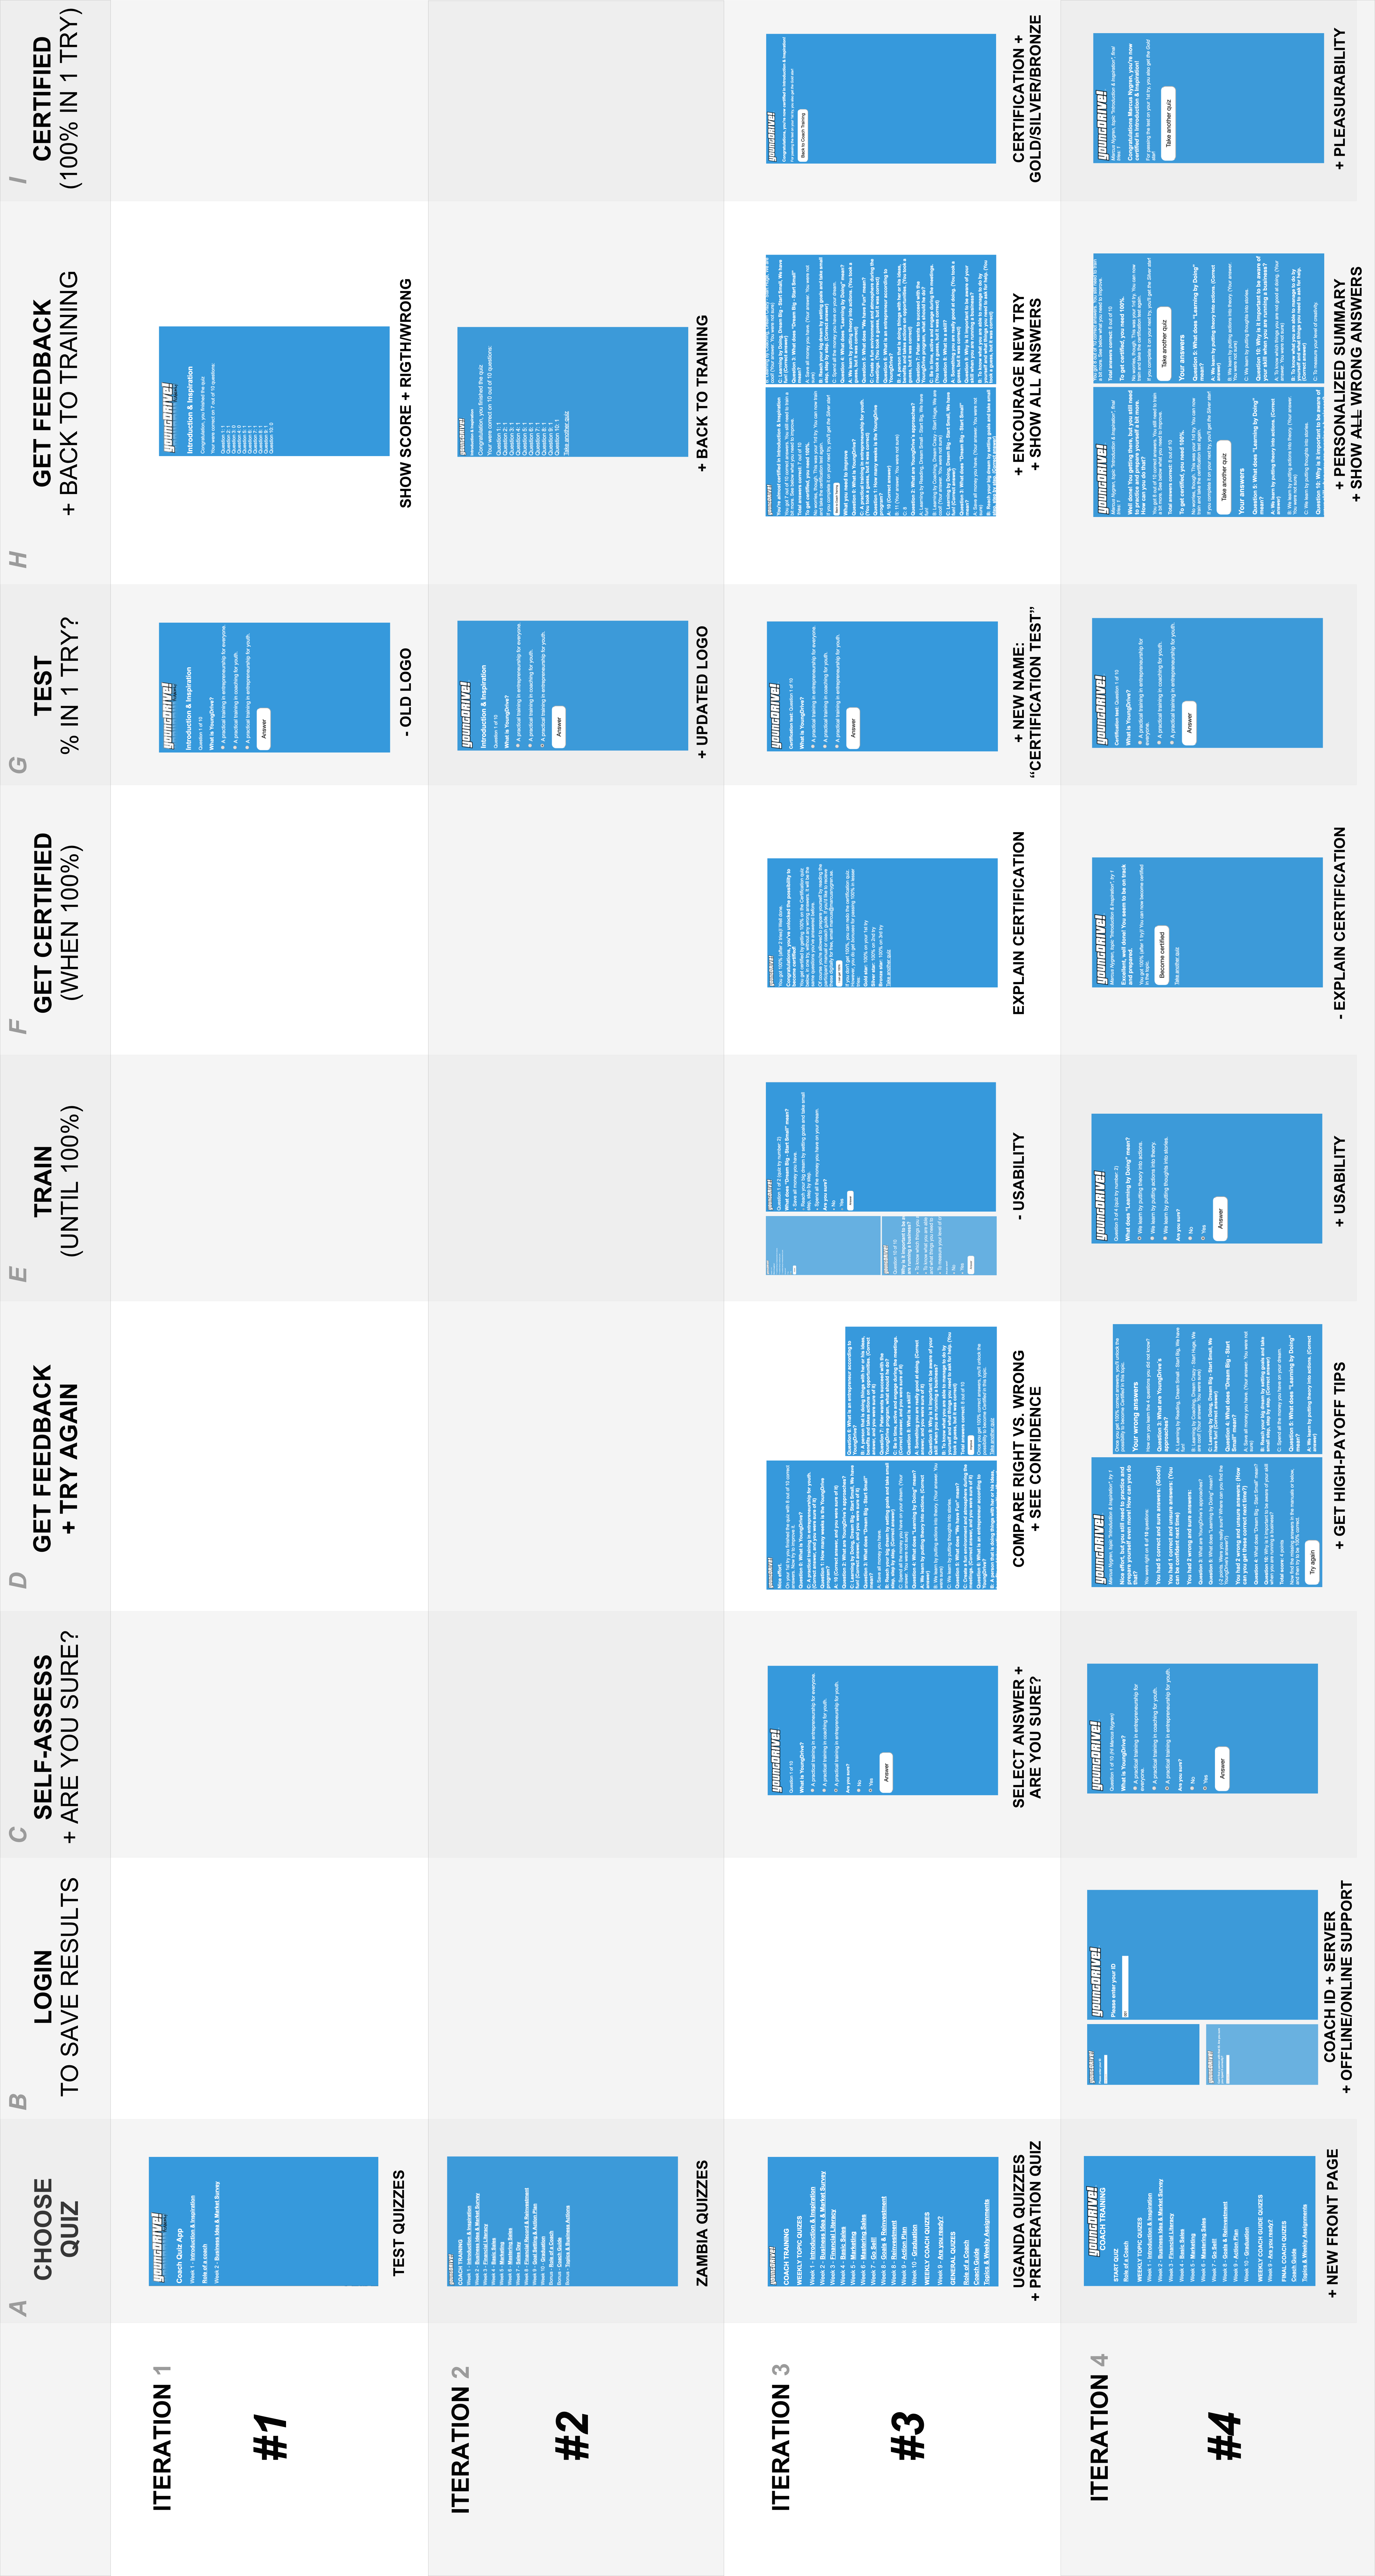
\includegraphics[width=1.0\textwidth]{IterationMapLowRes.png}
    \caption{The app flow described as a timeline (A-I), per iteration (1-4). E.g. in iteration 4, login (B4) appears after choosing quiz to take (A4).}
    \label{fig:iteration-map}
  \end{figure}

  %\subsection{Iteration \#1}

  There was no developed application at this point.


  The quiz flow during iteration 1-2 was a standard multiple-choice quiz game, designed for assessment, but not for learning. In a scoreboard, they could see which questions they were awarded points for and not, with a total score, see figure \ref{fig:iteration-map} H-1. In the end of iteration 2, whey were encouraged to go back to the start screen, to redo the same quiz again, or select a new one. 1 point is awarded for correct answers, whereas 0 points is given for incorrect answers.

  In iteration 3, feedback for self-reflection was introduced. The coach answers Yes or No on "Are you sure?" for each question (figure \ref{fig:iteration-map} C-3), with the aim of increasing meta-cognitive skills, and being able to give personalized feedback in the score board.

  Thanks to recording both if they were correct and confident, the app can give very precise learning feedback (e.g. showing that the coach answered alternative B with confidence, but showing that A was actually the correct alternative).

  In iteration 3-4, after observing their incorrect answers, and learning their correct ones (closely compare figure \ref{fig:iteration-map} D-3 and E-3), they could retake the wrong answers immediately.

  In iteration 3, the score board was simply showing each correct question with the answer the coach provided versus the correct one. After giving feedback, the coach can train, and improve on incorrect answers and guesses, and when being 100\% correct and confident, ideally take the whole quiz without faults.

  For iteration 4, the score board is more personal, encouraging the coach to reflect on her own learning process. The feedback is designed to give a self-confidence boost ("You were correct, and you were sure" or "You guessed, but you were correct. You can answer with confidence the next time"), unlearn knowledge ("You were incorrect, but you were sure"), or encourage studying more when unsure and wrong ("You were incorrect, and you were not sure").

  To discourage guessing during training, since iteration 3, the coach is shown number of tries on the quiz if they do not get 100\% in their first try (see the top bar of figure \ref{fig:iteration-map} E-3). For iteration 4, the coach will also get a minus point (-1) for answering incorrectly but confidently "Are you sure?": "Yes". If uncertain, the coach should answer "Are yo sure?": "No", and no penalty will be given. The coach will later recieve feedback, either "You can be confident next time" (if correct but unsure) or "How can you get these correct next time?" (if unsure and incorrect).

  The coach is encouraged to be well-prepared before trying again (either consulting the answers or the manuals). At 100\% correct answers, they can get certified, by getting the whole quiz correct without faults. Failing a question on the certification would show that they have not \textit{reliably} learned all the answers during the training. The more effort the coach has put into the training, the more likely the coach will be to pass the certification.

  %Lena Tibell menade vid förslaget att "Belöna inte hur snabbt %en elev går från att kunna till att inte kunna, för olika %människor lär sig olika snabbt". "Vad vi ville åstadkomma %med Antal försök var endast att undvika gissningarna".

   This certification quiz is the same as in training, but no longer do they need to answer "Are you sure?". If the coach can again get 100\% correct answers, without any faults, they have proved they are correct and confident with the topic they should teach the youth.

   If they fail a question, the score board will encourage more training and that they did not get certified, see figure \ref{fig:iteration-map} H-4. Since the coach did get 100\% correct in the training (maybe after a couple of tries) but not in the certification, the knowledge can be described as "Can do with effort". The coach can choose to take a new quiz, or take the same quiz from the beginning of the training.

   For passing the certification on the 1st, 2nd or 3rd time the coach is awarded a Gold, Silver or Bronze medal respectively (after certificate try 3, no medal is given, only the certificate). Compare figure \ref{fig:iteration-map} I-3 to I-4: for iteration 4, the "certificate" mentions the persons name and the topic certified in, which is a form of gamification in addition to the intrisic motivation of rewarding deliberate practice.
